\section{Non-flow correlations}
\label{secks:nonflow}
In this section various types of particle correlations, which are not caused by a collective behaviour developed in strongly interacting matter, are discussed. These are typically two-, or a few-, particle correlations arising due to a quantum interference, an interaction between the particles, a common source of production, such as a resonance decay, and a string or (mini-)jet fragmentation. The study of this type of correlations gives information about the space--time evolution of the system, and may shed light on particular production mechanisms.
\subsection{Femtoscopic correlations}
\label{subsecks:femto}
The term femtoscopy is often employed to indicate methods to measure spatial and time scales at a ${\cal O}(1)$~fm level. Basically, two effects are exploited: interference between identical particles and final state particle interactions. The identical-particle interference is consequence of the symmetrization of the wave function. It is connected to the Hanbury-Brown and Twiss (HBT) method proposed to measure stellar sizes~\cite{HanburyBrown:1954wr}, therefore it is sometimes called also in the heavy-ion field HBT method. The production of identical bosons (e.g. pions) with close momenta will be enhanced by such an effect, and that of identical fermions (e.g. protons) will be suppressed. The correlation length in the momentum space is inversely proportional to the spatial size of the source region, assuming that the particles are emitted incoherently. However, the measured correlation is affected by other effects, such as Coulomb interactions, resonance decays, and final state particle interactions, which have to be duly taken into account in the analyses. The latter effect, being often of a short-range nature and present also for non-identical particles, can itself be exploited for femtoscopic studies.

The first results were obtained for like-sign pion--pion correlations with early Pb--Pb data at the LHC~\cite{Aamodt:2011mr}. The analysis was performed in three dimensions, decomposing the relative momentum between the two pions in the longitudinally co-moving system (centre-of-mass system boosted along the beam direction such that the two-pion longitudinal momentum is zero) into its `out' (direction of the momentum of the pion pair), `side' (direction perpendicular to the pair momentum and the beam axis), and `long' (along the beam axis) components. The like-sign two-particle distribution in the three-dimensional relative momentum is normalized to that obtained for pairs of particles from different events (event mixing). At small relative momentum the correlation function exhibits the Bose--Einstein enhancement peak, which is fitted with an expression accounting for the incoherent pion emission from a three-dimensional Gaussian-density source and Coulomb repulsion between particles. As a result the Gaussian HBT radii $R_{\rm out}$, $R_{\rm side}$, and $R_{\rm long}$ are extracted. The analysis is performed as a function of $k_{\rm T}$ (one-half of the total pair transverse momentum). The HBT radii are found to be significantly larger (by 10--35\,\%) than those measured at RHIC~\cite{Adams:2004yc}, and show a decreasing trend with increasing $k_{\rm T}$, as also observed in heavy-ion collision experiments at lower energies~\cite{Lisa:2005dd}. This is a characteristic feature of expanding particle sources since the HBT radii describe the homogeneity length rather than the overall size of the particle emitting system. The homogeneity length is defined as the size of the region that contributes to the pion spectrum at a particular momentum.

\begin{figure}
\centering
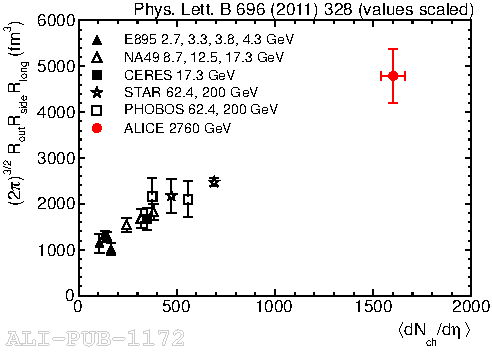
\includegraphics[width=0.5\textwidth]{ksfigures/HBTVolumeVsDensity.pdf}
\caption{Homogeneity volume for $k_{\rm T} = 0.3$~GeV as a function of the charged-particle density, measured in heavy-ion collisions at different energies. Adapted from~\cite{Aamodt:2011mr}.}
\label{figks:HBTvolume}
\end{figure}

The energy dependence of the HBT radii is usually expressed as a function of the cubic root of the charged-particle pseudorapidity density, i.e. as $({\rm d}N_{\rm ch}/{\rm d}\eta)^{1/3}$. The approximately linear increase (at a given $k_{\rm T}$) is well-described by hydrodynamical calculations~\cite{Chojnacki:2007rq,Karpenko:2009wf}. The product of the three radii, measured at different energies at $k_{\rm T} = 0.3$~GeV, is shown in Fig.~\ref{figks:HBTvolume} as a function of the charged-particle pseudorapidity density ${\rm d}N_{\rm ch}/{\rm d}\eta$. This product, multiplied by a factor $(2\pi)^{3/2}$ due to Gaussian distribution normalization, representing then the homogeneity volume, increases linearly with the particle density. At the LHC the homogeneity volume for pion emission for the 5\,\% most central Pb--Pb collisions doubles compared to that at the top RHIC energy. Within a hydrodynamic scenario the decoupling time for hadrons ($\tau_{\rm f}$, corresponding to kinetic freeze-out) can be extracted from the $k_{\rm T}$ dependence of $R_{\rm long}$ ($\tau_{\rm f} \propto R_{\rm long}$)~\cite{Herrmann:1994rr}. The decoupling time, estimated this way for different collision energies, is presented in Fig.~\ref{figks:HBTtime}. It increases linearly with $({\rm d}N_{\rm ch}/{\rm d}\eta)^{1/3}$, and reaches for most central LHC collisions a value by a factor 1.4 larger than was observed at RHIC. Note that the estimate for $\tau_{\rm f}$ was done for an assumed kinetic freeze-out temperature $T_{\rm kin} \approx 120$~MeV, if one were to use the latest measured value (Sec.~\ref{subsecks:identspectra}), the decoupling time would increase to 13--14~fm.

\begin{figure}
\centering
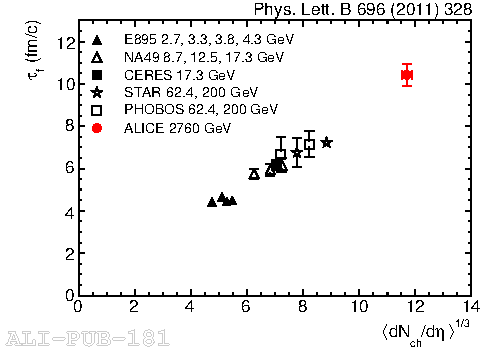
\includegraphics[width=0.5\textwidth]{ksfigures/HBTDecouplTime.pdf}
\caption{Decoupling time as a function of the cube root of charged-particle pseudorapidity density, measured in heavy-ion collisions at different energies. Reproduced from~\cite{Aamodt:2011mr}.}
\label{figks:HBTtime}
\end{figure}

In the study of two-pion correlations, the assumption was that the pion emission is incoherent, i.e. the source is fully chaotic. In such conditions the strength of the Bose--Einstein correlations is maximal, and would decrease for a source with a lower degree of chaoticity. Such a situation may be created in heavy-ion collisions, if some kind of condensate would be present or formed (e.g. colour-glass condensate, disoriented chiral condensate). The degree of chaoticity can be assessed comparing two- and three-pion correlations. A recent analysis~\cite{Abelev:2013pqa} found that the genuine three-pion correlation is suppressed relative to the two-pion correlation, assuming fully chaotic pion emission. This suppression decreases with pion-triplet momentum, and at low momentum (pion $p_{\rm T} \sim 0.3$~GeV) may correspond to a coherent fraction in charged pion emission of $(22 \pm 12)$\,\%.


%HBT sizes vs particle density
%volume vs energy
\subsection{Fluctuations}
\label{subsecks:fluct}
Study of event-by-event fluctuations provides a tool to characterize the thermodynamic properties of the system. Such fluctuations are also affected by the system evolution. The fluctuations of conserved quantities in a finite phase space window, such as the net charge of the system described in~\cite{Abelev:2012pv}, are predicted to be sensitive signals of QGP formation and of the phase transition and may provide an important insight on the properties of strong interactions. In the QGP phase, the charge carriers are quarks with their fractional charges, whereas particles in the hadron phase carry unit charge. The fluctuations in the net charge depend on the squares of the charge states present in the system. Consequently, the net-charge fluctuations in the QGP phase are expected to be significantly smaller compared to those in the hadron phase. The event-by event fluctuations of the net charge in a specific phase-space window (for example a given pseudorapidity interval around mid-rapidity) are usually quantified by the $D$ variable~\cite{Jeon:2000wg}, defined as:
\begin{equation}
D = \langle N_{+} + N_{-} \rangle \langle \delta (N_{+} / N_{-})^2 \rangle \approx 4 \langle \delta (N_{+} - N_{-})^2 \rangle / \langle N_{+} + N_{-} \rangle .
\end{equation}
Here $N_{+,-}$ are the numbers of particles of the two charges in that window, angle brackets denote the average value over the ensemble of events, and $\delta$ indicates the variance of the quantity under the square sign. The value of $D$ measures the fluctuation of the net charge ($N_{+} + N_{-}$) per entropy unit, and is predicted to be around 3 for hadron gas and significantly lower, 1--1.5, for the QGP phase~\cite{Jeon:2003gk}. Figure~\ref{figks:ChargeFluct} presents the energy dependence of the D measure obtained by the STAR experiment~\cite{Abelev:2008jg} at RHIC and by ALICE at the LHC in the most central collisions. The fluctuations are expected to be diluted during the medium evolution and thus the D measure may not reach the value predicted for the QGP phase, however, a clear tendency going closer to that prediction with increasing energy is observed.

\begin{figure}
\centering
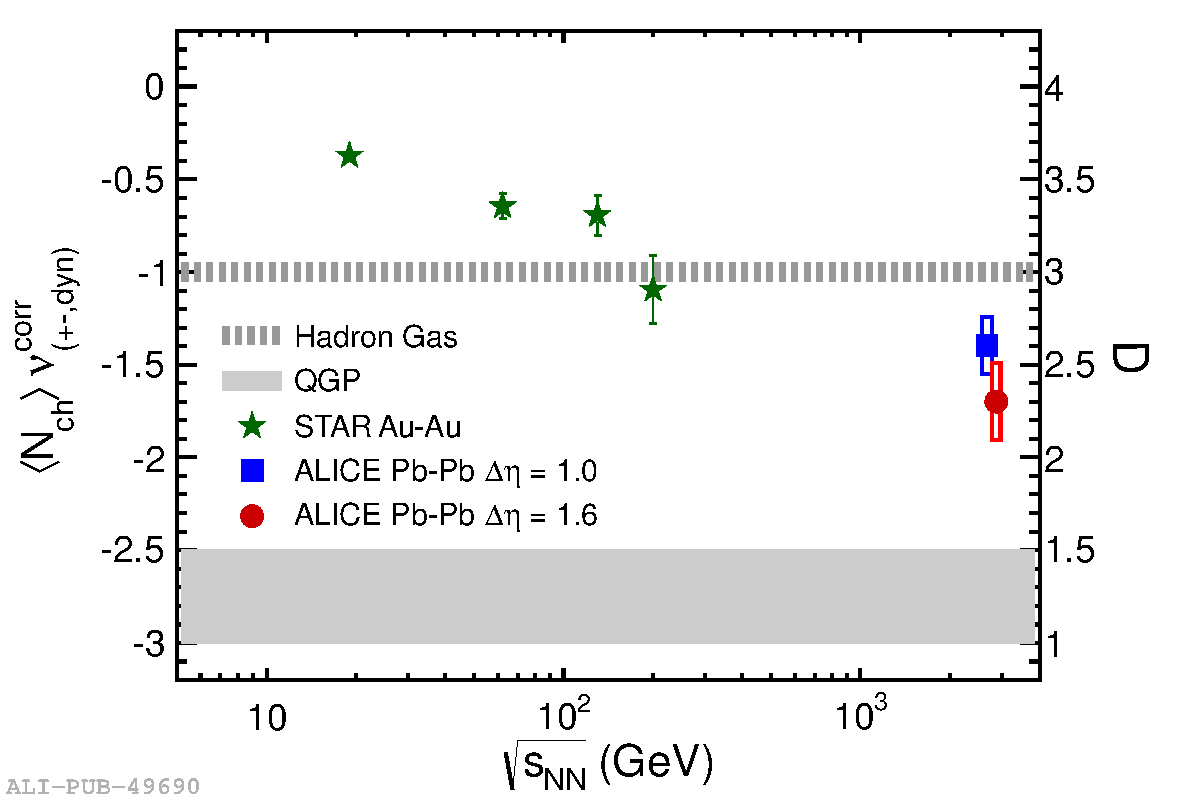
\includegraphics[width=0.5\textwidth]{ksfigures/NetChargeFluct.pdf}
\caption{Energy dependence of net-charge fluctuations represented as D-measure (defined in the text) in the most central collisions. The two ALICE measurements are for two different pseudorapidity intervals $\Delta\eta$ centred around mid-rapidity, and the STAR results are for $\Delta\eta = 1$. The D values are shown on the right-hand ordinate and the shaded areas correspond to the two predictions according the legend. The quantity of the left-hand side ordinate represents the way how the D values are measured, and it is not discussed here. Reproduced from~\cite{Abelev:2012pv}.}
\label{figks:ChargeFluct}
\end{figure}

Event-by-event fluctuations of the mean transverse momentum of charged particles are studied as a function of the charged-particle multiplicity in Pb--Pb collisions with the ALICE experiment, and significant non-statistical fluctuations are observed. The dynamical mean $p_{\rm T}$ fluctuations arise from correlations among the $p_{\rm T}$ of the final-state particles, e.g. due to resonance decays, jets, or quantum correlations. To account for such conventional contributions, similar studies are performed in pp, where these correlations are also present.  These fluctuations are expected to decrease with increasing particle density (collision centrality), as $({\rm d}N_{\rm ch}/{\rm d}\eta)^{-1/2}$ under the assumption of independent sources. The measured dependence for peripheral collisions (corresponding to centrality percentiles in the range 60--90\,\%) follows the pp extrapolation, however, already there the particle-density dependence has a power close to $-0.4$ instead of $-1/2$. This is interesting, because significant differences in the mean $p_{\rm T}$ are observed between pp and Pb--Pb in that multiplicity range~\cite{Abelev:2013bla}. At larger particle densities the Pb--Pb fluctuation results deviate from the pp extrapolation: an enhancement in the 40--60\,\% centrality range is followed by a pronounced decrease for more central events, which indicates a strong reduction of fluctuations towards central collisions. This centrality dependence is compatible with that observed at RHIC~\cite{Adams:2005ka}. The Pb--Pb data can not be described by models based on independent nucleon--nucleon collisions such as HIJING~\cite{Wang:1991hta,Deng:2010xg}. Models which include initial state density fluctuations and their effect on the development of collectivity in the final state such as AMPT~\cite{Lin:2004en} are in reasonable qualitative agreement with the data. This suggests a connection between the observed transverse momentum fluctuations and azimuthal correlations, and their relation to fluctuations in the initial state of the collision.

%charge particle balance function
\subsection{Angular correlations}
\label{subsecks:angular}
The angular correlations between two particles are widely used to study various phenomena of both non-flow and collective-flow origin. Here, the method and some applications to non-flow studies is described. The exploitation of the angular correlations for investigation of the azimuthally-dependent flow is explained in Sec.~\ref{sec:ps:flow}. The two-particle correlation between pairs of particles is measured as a function of the azimuthal difference $\Delta\varphi$ (defined usually within $−\pi/2$ and $3\pi/2$) and pseudorapidity difference $\Delta\eta$. Various kinds of particle pairs are used: they can be all charged particles, pairs selected by charge (like sign, unlike sign), pairs when one particle (trigger) has given $p_{\rm T}$ or type while the second particle (associated) may have some other characteristics, etc. The two-dimensional distribution is constructed for pairs of particles from the same event, and basically two types of the normalization are used: each event is normalized (per number of pairs, or number of triggers) and then the events are summed up, or the events are first summed up and then normalized to the total number (of pairs or triggers). Therefore, one has to be careful, when comparing the results from different experiments, which may have employed different normalization. Then a second two-dimensional distribution is constructed for pairs of particles from the different events (or a trigger particle form one event and all associated from another one). This mixed-event distribution is usually uniform in the $\Delta\varphi$ direction and has a triangular shape in the $\Delta\eta$ direction, reflecting the geometrical acceptance: maximum at $\Delta\eta = 0$, dropping to zero at $\Delta\eta = \pm$~the detector size in pseudorapidity. The second distribution is normalized to unity at its maximum (i.e. at $\Delta\eta = 0$), and then used to divide the normalized distribution obtained for particle pairs from the same event. In this way, the acceptance and detection efficiency are taken into account.

\begin{figure}
\centering
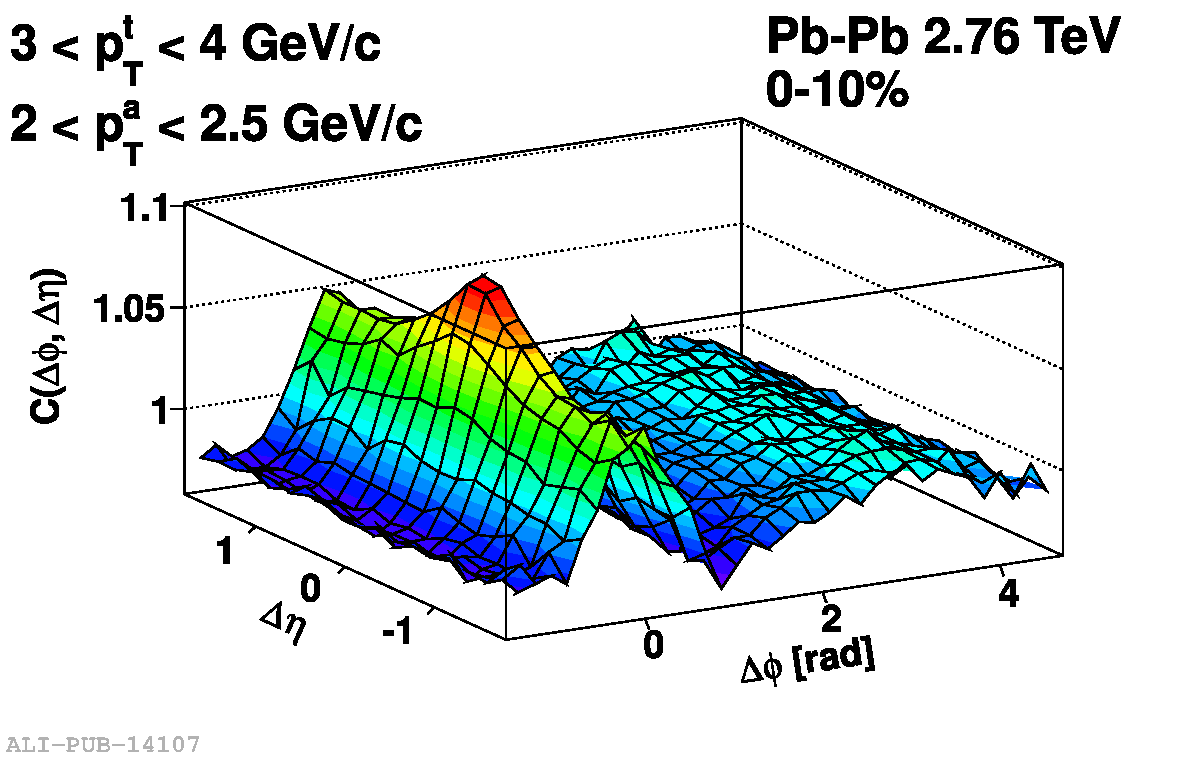
\includegraphics[width=0.5\textwidth]{ksfigures/TwoParticleCorrFunction.pdf}
\caption{Example of the two-particle correlation function in $\Delta\varphi$ and $\Delta\eta$ for trigger and associated particle selected in $p_{\rm T}$ intervals displayed in the upper-left corner. The top 10\,\% of most central Pb--Pb collisions are used. Reproduced from~\cite{Aamodt:2011by}.}
\label{figks:CorrExamle}
\end{figure}


An example of such two-dimensional two-particle particle correlation is illustrated in Fig.~\ref{figks:CorrExamle}. This is obtained for trigger--associated particle pairs selected according their $p_{\rm T}$ as indicated in the figure. Some typical structures are apparent:
\begin{itemize}
 \item{the peak around $(\Delta\varphi,\Delta\eta) = (0,0)$ is due to (mini-)jets, sometimes a much narrower peak is also visible on top of that, caused by HBT correlations (for like-sign pairs), or by gamma conversions (for unlike-sign pairs);}
 \item{the near-side ridge at $\Delta\varphi = 0$ continuing from the jet peak along the $\Delta\eta$ direction to larger $\Delta\eta$ values, this is presumably caused by the elliptic and higher-harmonic flow (see Sec.~\ref{sec:ps:flow};}
 \item{the away-side ridge at $\Delta\varphi = \pi$ along the $\Delta\eta$ direction, where the second jet may appear (often quenched), now spread along $\Delta\eta$ because the parton--parton system at the origin of the two jets moves longitudinally with respect to the collision centre-of-mass system, in addition the flow azimuthal modulation also contributes here.}
\end{itemize}
The angular two-particle correlations are analyzed by studying their centrality development, and often by projecting them on one of the axes, excluding or not some structures discussed above.

The two-particle correlations are used to study parton quenching at $p_{\rm T}$ below ${\cal O}(10)$~GeV~\cite{Aamodt:2011vg}, where the full jet reconstruction is difficult due to background fluctuations~\cite{Abelev:2012ej}. In the example shown here the selection requires: a trigger within $8 < p_{\rm T}^{\rm t} < 15$~GeV while the associated $p_{\rm T}^{\rm a}$ is a variable parameter, respecting $p_{\rm T}^{\rm a} <p_{\rm T}^{\rm t}$. The two-dimensional correlation is projected on the $\Delta\varphi$ axis in order to measure the number of associated particles correlated to the trigger particle in the near-side and the away-side jet structures. The background from the underlying event, possibly modulated by elliptic flow, has to be subtracted. This is done using three methods: a flat background obtained by the ZYAM (Zero Yield At Minimum) method (the minimum between the near- and the away-side peaks is used to evaluate the background level), a background modulated according the available elliptic-flow $v_2$ measurements, and a flat background estimated according to the value in the region $|\Delta\varphi| < \pi/2$ and $|\Delta\eta| > 1$  ($\Delta\eta$-gap). After background subtraction the distribution is integrated around the near- and away-side peaks, in the $\pm 0.7$ and $\pi \pm 0.7$ $\Delta\varphi$ intervals, respectively. The per-trigger yields of associated particles, obtained this way, are normalized to the same yields measured in pp collisions. Such a ratio is denoted $I_{\rm AA}$ and it represents the nuclear modification factor of the conditional yields. In Fig.~\ref{figks:IAA} the near- and away-side $I_{\rm AA}$ are presented as a function of associated-particle $p_{\rm T}^{\rm a}$ for peripheral and central Pb--Pb collisions. The results are practically independent on $p_{\rm T}^{\rm a}$, and for peripheral collisions compatible with unity, i.e. no nuclear modification is observed. For central collisions, the away-side $I_{\rm AA}$ is around 0.6, which is interpreted as a manifestation of jet quenching. On the near-side the $I_{\rm AA}$ is above unity, such an effect was not observed at lower energies. The near-side enhancement could be understood as due to a modification of the fragmentation function, possibly caused by jet quenching and a trigger bias. This measurement constrains various models, some of those showed to be capable to describe such an enhancement~\cite{Renk:2011wp}.

\begin{figure}
\centering
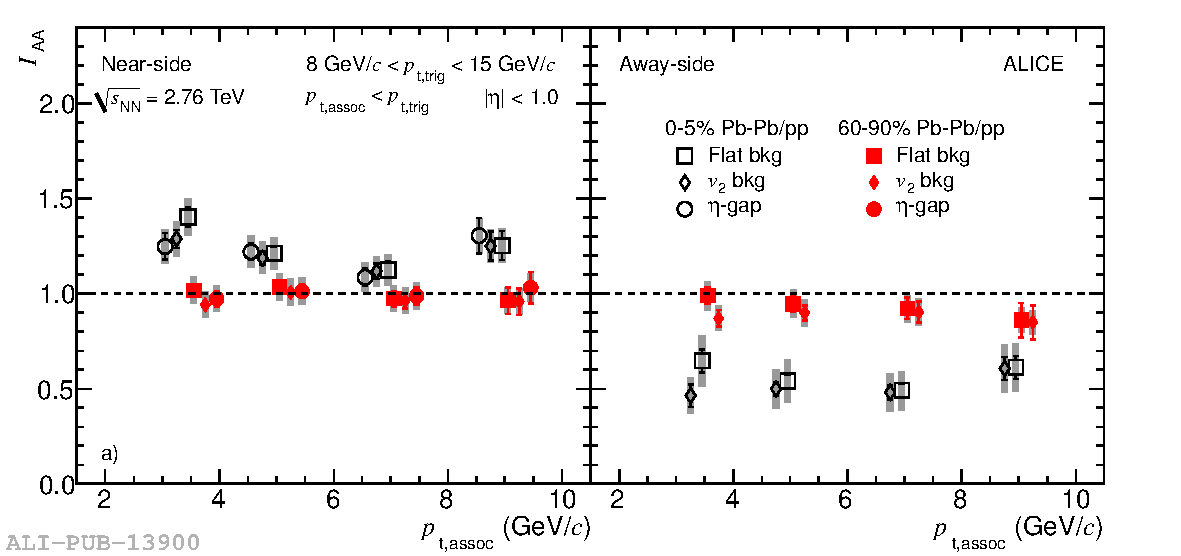
\includegraphics[width=0.7\textwidth]{ksfigures/IAA.pdf}
\caption{Near-side (left) and away-side (right) $I_{\rm AA}$ as a function of the transverse momentum of associated particles. The results are shown for peripheral (60--90\,\%) and central (0--5\,\%) Pb--Pb collisions. The three values shown for each measurement correspond to the three background subtraction methods described in the text. Reproduced from~\cite{Aamodt:2011vg}.}
\label{figks:IAA}
\end{figure}

The jet-shape studies measuring the jet-structure widths in $\Delta\varphi$ and $\Delta\eta$ directions, exploited the triggered two-particle correlations as well. It was reported that the $\Delta\eta$ jet-structure size increases for more central Pb--Pb collisions, while in the $\Delta\varphi$ direction such an increase, if any, is much smaller. This could be explained by an interaction of the jet with longitudinally flowing medium. The particle composition of the jet-like structure was also studied. The p/$\pi$ ratio is measured in $(\Delta\varphi, \Delta\eta)$ regions, both outside and inside the jet structures selected in the correlation plot. Correcting the jet region with properly weighted outside-jet measurement, the p/$\pi$ ratio for the jet structure is obtained. While the outside-jet p/$\pi$ ratio reproduces the heavy-ion baryon anomaly (see Sec.~\ref{subsecks:identspectra}), the result for the jet structure is compatible with the expectation for the jet fragmentation in pp collisions.

\begin{figure}[!ht]
\centering
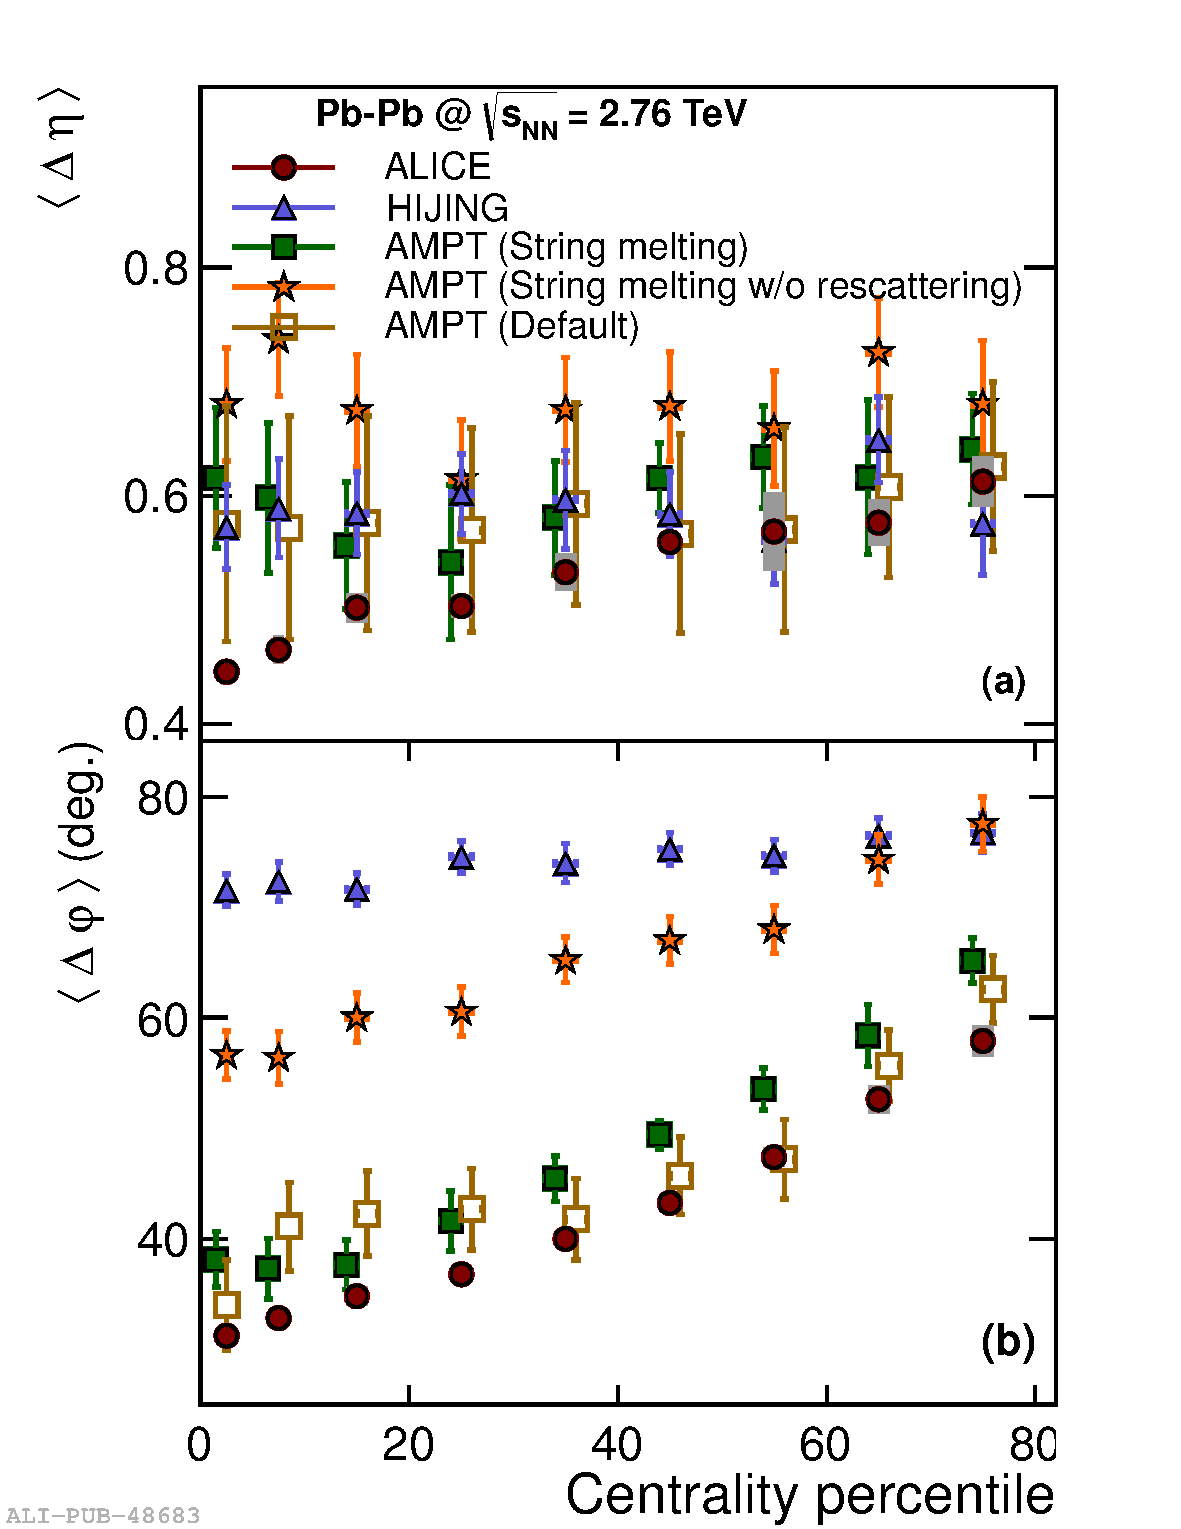
\includegraphics[width=0.5\textwidth]{ksfigures/BalanceFunctionWidth.pdf}
\caption{Charge balance function widths in longitudinal (upper part - a) and azimuthal (lower part - b) directions as a function of collision centrality, expressed in percentiles. Model calculations are presented with markers according to the legend. Reproduced from~\cite{Abelev:2013csa}.}
\label{figks:Balance}
\end{figure}

The study of the charge balance function is performed using the correlations constructed for unlike-sign and like-sign particle pairs separately~\cite{Abelev:2013csa}. The balance function is defined as one half of the difference between the unlike-sign and like-sign correlations, and measures the distance over which the charge of particles is compensated. The widths of the balance function in the two directions, $\langle \Delta\varphi \rangle$ and $\langle \Delta\eta \rangle$, are shown in Fig.~\ref{figks:Balance} as a function of the collision centrality. The measurement indicates that the charge is compensated in both directions on a shorter scale for more central collisions. Such behaviour was already observed at RHIC~\cite{Aggarwal:2010ya}, however, the $\langle \Delta\varphi \rangle$ and $\langle \Delta\eta \rangle$ values are significantly larger at the LHC. The model calculations~\cite{Wang:1991hta,Lin:2004en} presented in Fig.~\ref{figks:Balance} have difficulties to reproduce the centrality dependencies in both directions.

\subsection{Chiral magnetic effect}
\label{subsecks:chiral}
Under the influence of the strong magnetic field along the direction of the angular momentum generated by the colliding nuclei, the quark spin alignment and the imbalance of the left- and right-handed quarks, would generate an electromagnetic current~\cite{Kharzeev:2004ey,Fukushima:2008xe,Kharzeev:2007jp}. Subsequent quark fragmentation into charged hadrons may induce a charge separation along the direction of the magnetic field (perpendicular to the reaction plane, defined by the beam axis and the centres of the colliding nuclei). This phenomenon is called the Chiral Magnetic Effect (CME). Azimuthal correlations among particles provide a powerful tool for the experimental study of particle production with respect to the reaction plane~\cite{Abelev:2012pa}.

Let's denote by $\psi_\pm$ the azimuthal angle of a particle of given charge with respect to the reaction plane. The orientation of the reaction plane itself is estimated by different techniques used in the studies of azimuthal asymmetry, Sec.~\ref{sec:ps:flow}. The multi-particle correlator $\langle \cos{(\psi_{\pm,\alpha} + \psi_{\pm,\beta})} \rangle$ (`multi-particle' because it depends on the reaction-plane angle, determined with other particles) probes the magnitude of the parity-odd amplitude possibly present in the azimuthal distribution with respect to the reaction plane~\cite{Voloshin:2004vk}. Such correlator also suppresses the background (non-flow) correlations unrelated to the reaction plane. It can be expressed as the difference of two terms: $\langle \cos{\psi_{\pm,\alpha}} \cos{\psi_{\pm,\beta}} \rangle$ and $\langle \sin{\psi_{\pm,\alpha}} \sin{\psi_{\pm,\beta}} \rangle$, the latter term quantifies the out-of-plane (i.e. in the direction of magnetic field) charge correlations sensitive to the CME. In order to evaluate the two terms separately, the two-particle correlator $\langle \cos{(\psi_{\pm,\alpha} - \psi_{\pm,\beta})} \rangle$ is used, which is independent of the reaction plane angle, however, susceptible to large background contributions. This second correlator is equal to the sum of the two terms mentioned above. It should be mentioned that both correlators could be affected by other effects, such as momentum conservation, local charge conservation, and fluctuations in the initial energy density.

\begin{figure}
\centering
%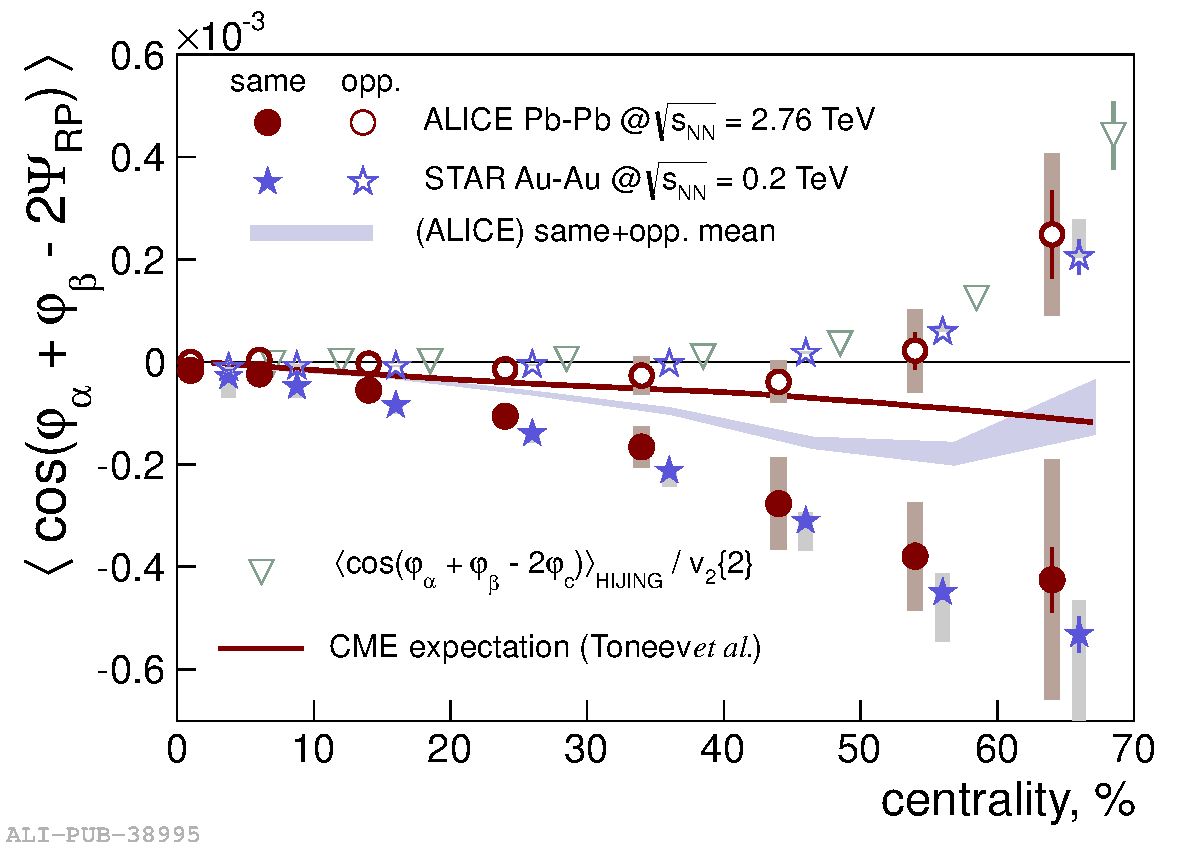
\includegraphics[width=0.5\textwidth]{ksfigures/ChargeSepar.pdf}
\caption{Centrality dependence of the multi-particle correlator defined in text as $\langle \cos{(\psi_{\pm,\alpha} + \psi_{\pm,\beta})} \rangle$. The ALICE results are obtained from the cumulant analysis.  The triangles represent the three-particle correlations from HIJING~\cite{Wang:1991hta} corrected for the experimentally measured $v_2$. A model prediction for the like-sign correlations incorporating the chiral magnetic effect for LHC energies~\cite{Toneev:2010xt} is shown by the solid line. The shaded band represents the centrality dependence of the charge independent correlations. Reproduced from~\cite{Abelev:2012pa}.}
\label{figks:ChSep}
\end{figure}


The centrality dependence of the multi-particle correlator $\langle \cos{(\psi_{\pm,\alpha} + \psi_{\pm,\beta})} \rangle$ for like-sign (labeled as `same') and unlike-sign (labeled as `opp.') particle pairs is presented in Fig.~\ref{figks:ChSep}. The contribution from the CME to the correlations of like-sign and unlike-sign pairs is expected to be similar in magnitude and opposite in sign, however, these correlations could be modified by the medium, that may result in the dilution of the correlations for unlike-sign particles. The LHC results are (unexpectedly) compatible with the RHIC measurements~\cite{Abelev:2009ac}. This is not true for the second (two-particle) correlator, may be due to different background contributions. In Fig.~\ref{figks:ChSep} the experimental results are compared to a model prediction for like-sign correlations~\cite{Toneev:2010xt}, which predicts a significantly smaller effect at the LHC than at RHIC. The magnitude of the effect and its energy dependence crucially rely on the duration and time evolution of the magnetic field, which is at present a matter of intense discussions. To conclude, a clear signal compatible with a charge-dependent separation relative to the reaction plane is observed and can be used to constrain theoretical calculations.
